\documentclass{article}
\usepackage{../tex/mysty}
\usepackage[final]{pdfpages}
\begin{document}


\maketitlepage{U.S. Food and Drug Administration: Regulatory
  Report}{Sanjay Challa}

\setcounter{tocdepth}{3}
\tableofcontents
\newpage

\section*{Executive summary}
\label{sec:exec-summary}

\section{Regulation Overview}
\label{sec:test-administration}

\section{Device Classification}
\label{sec:protocols}


\addcontentsline{toc}{section}{510(k) Premarket Notification}
% Cover sheets
\addcontentsline{toc}{subsection}{CDRH Premarket Review Submission Cover Sheet}

\begin{figure}[H]
  \centering
  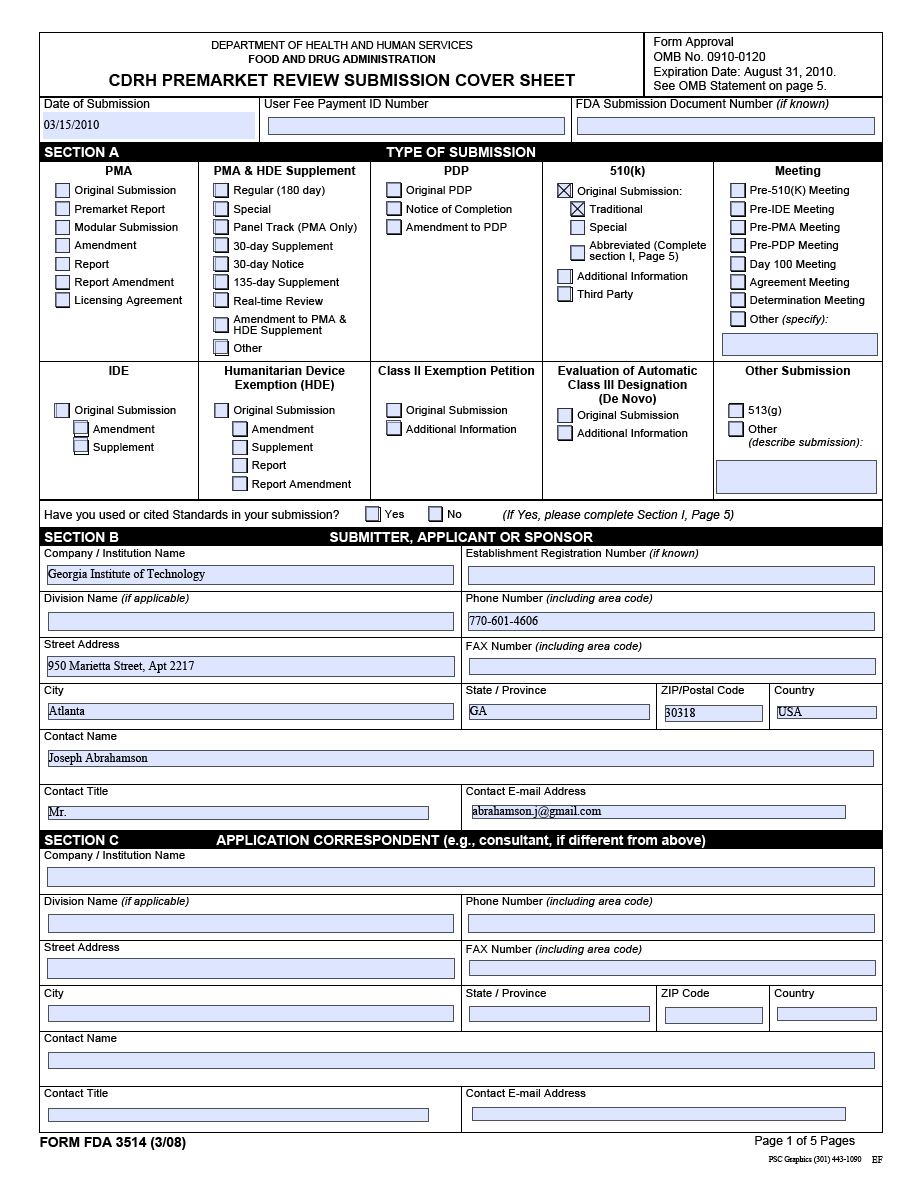
\includegraphics[width=1.2\linewidth]{pages/cdrh-pics/1}
  \label{fig:summary}
\end{figure}

\begin{figure}[H]
  \centering
  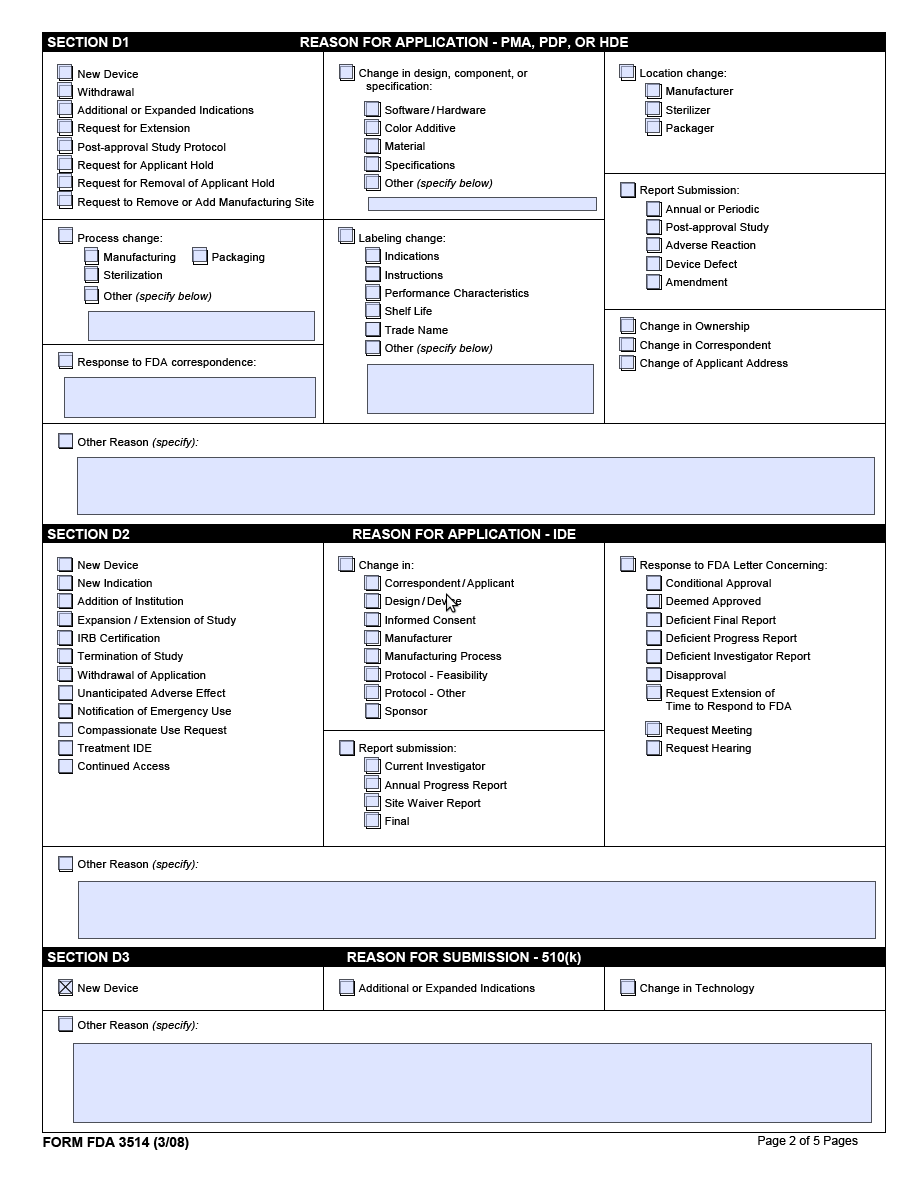
\includegraphics[width=1.2\linewidth]{pages/cdrh-pics/2}
  \label{fig:summary}
\end{figure}

\begin{figure}[H]
  \centering
  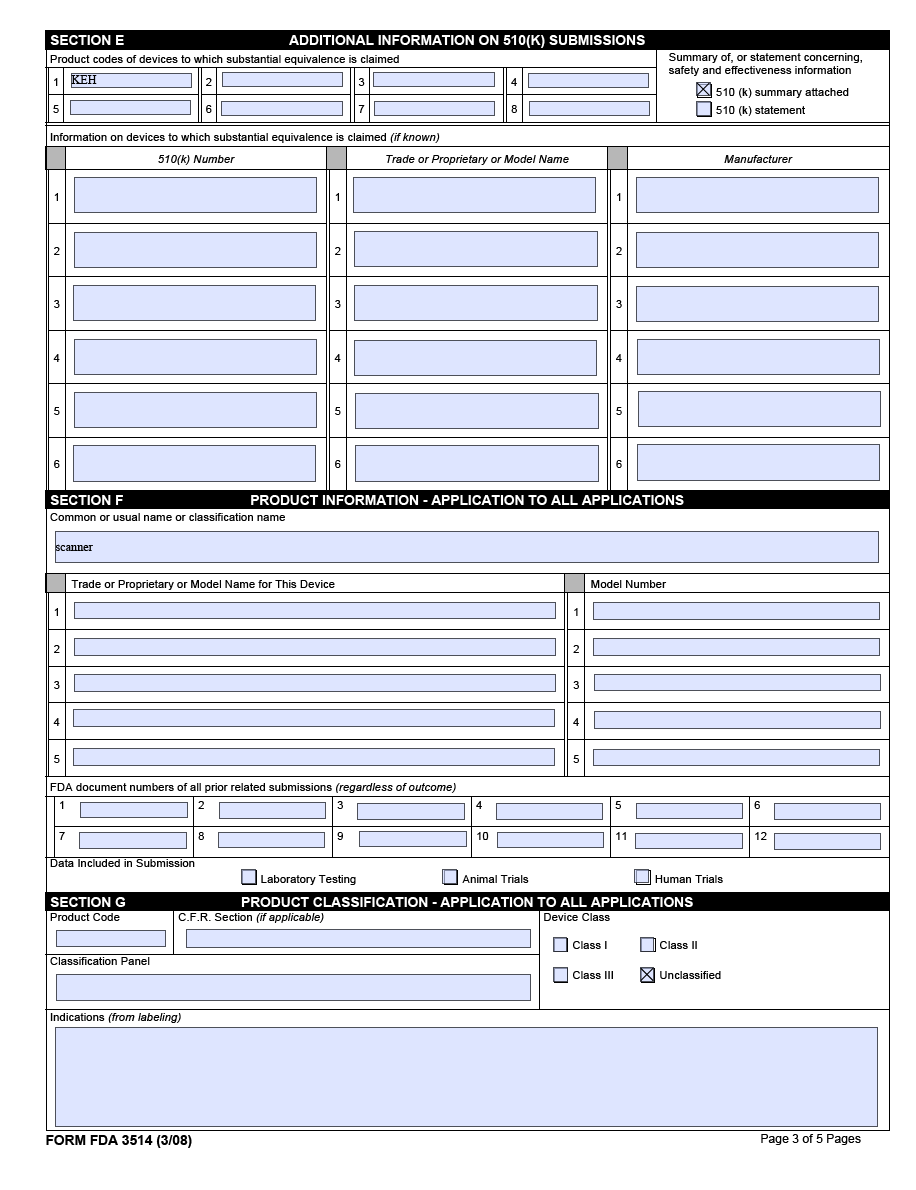
\includegraphics[width=1.2\linewidth]{pages/cdrh-pics/3}
  \label{fig:summary}
\end{figure}

\begin{figure}[H]
  \centering
  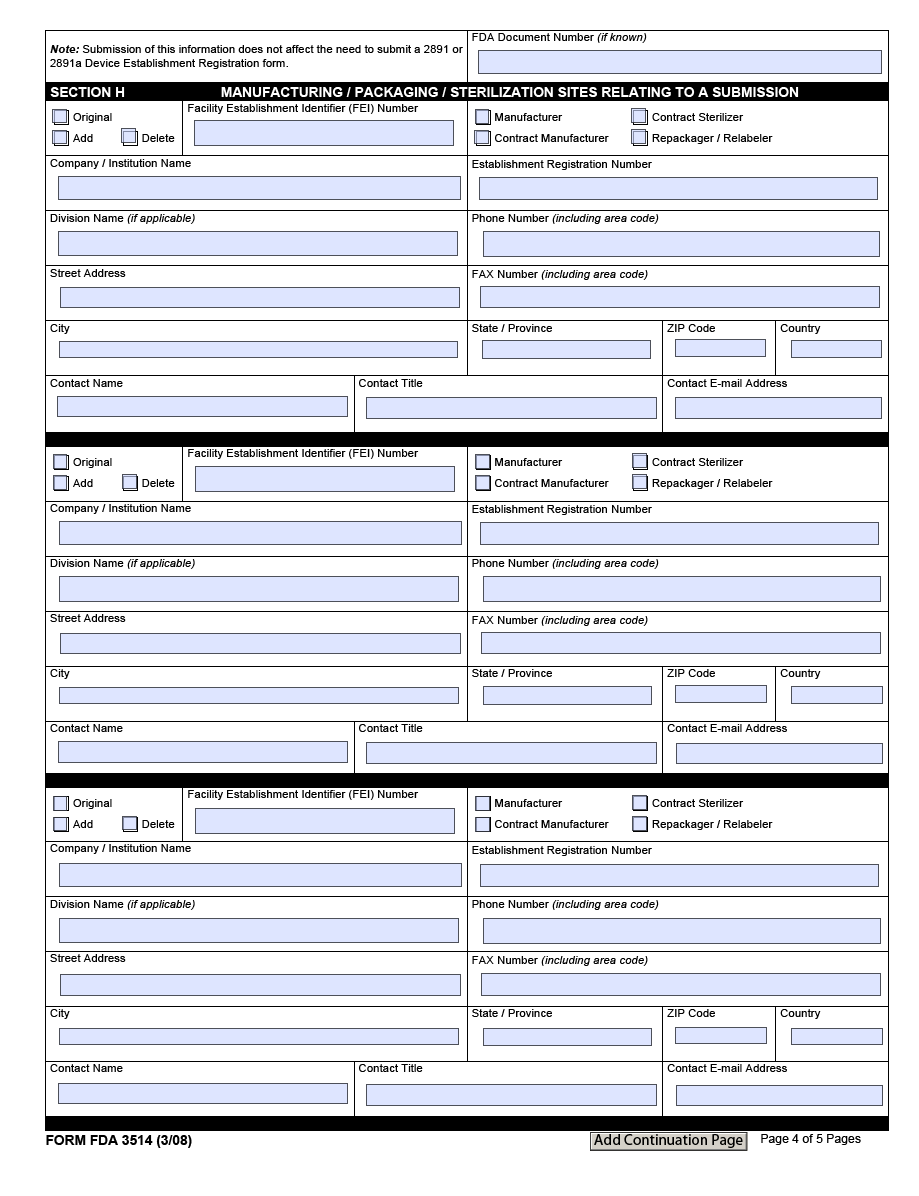
\includegraphics[width=1.2\linewidth]{pages/cdrh-pics/4}
  \label{fig:summary}
\end{figure}

\begin{figure}[H]
  \centering
  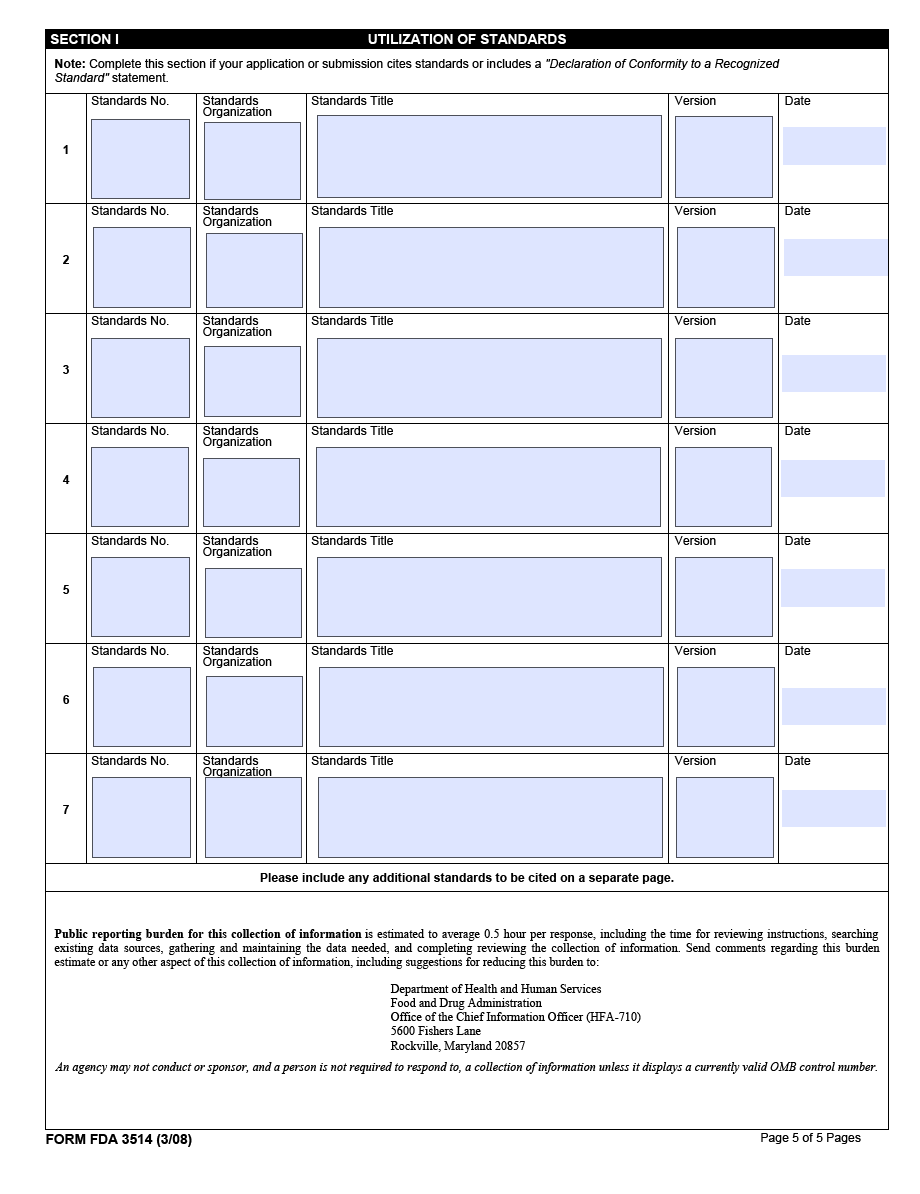
\includegraphics[width=1.2\linewidth]{pages/cdrh-pics/5}
  \label{fig:summary}
\end{figure}

%%% Local Variables: 
%%% mode: latex
%%% TeX-master: "../reg"
%%% End: 

\newpage
\addcontentsline{toc}{subsection}{510(k) Cover Letter}
\singlespacing

\begin{flushright}
  \huge{510(k) Submission --- Traditional}\\[.5in]
  
  \begin{minipage}{0.8\textwidth}
    \begin{flushright}
      \large \textbf{Scanner: eyeScan Mezzo} \\
      \textit{\today}
    \end{flushright}
  \end{minipage}
\end{flushright}

\begin{flushleft}
  Joseph Abrahamson\\
  $<$\textit{abrahamson.j@gatech.edu}$>$ \\
  Phone: 770 601 4606 \\[1em]
  
  \textit{Will register establishment following FDA clearance.}
\end{flushleft}
\vspace{4em}

\onehalfspacing

We seek FDA clearance to market our device, \textbf{eyeScan Mezzo}, a
Class II medical device used for medical scanning of three-dimensional
exterior eye shape. To our knowledge FDA has not classified this
device and, thus, no product code has been assigned or requested for
this device in the Classification Database. Substantially equivalent
devices belong to the General \& Plastic Surgery, Radiology, and
Pathology panels. This finished component is a novel device not
previously marketed with FDA clearance in the USA. We require 510(k)
clearance due to substantial equivalence with existent optical
coherence tomography devices (regulation no. \textbf{886.1570},
product code \textbf{OBO}), x-ray computed tomography devices
(regulation no. \textbf{892.1750}, product code \textbf{JAK}), and
microscopes, micrometers, and accessories (regulation
no. \textbf{864.3600}, product code \textbf{KEH}). Manufacturing
registration is currently unspecified. 

With regards to performance standards, this device contains electrical
components, and is subject to testing under IEC 60601-1-2 Part
I. Furthermore, the device contains a laser component, which under 21
CFR 1000 dictates that the device falls under RCHSA controls. RCHSA
controls indicate that the manufacture of the laser component of this
device is subject to standards 1002.10, 1002.13, and 1002.30, which
specifiy necessary reporting on the manufacturing of the laser
component. Lastly, while the device does contain a laser, it is exempt
from 21 CFR 1040.

%%% Local Variables: 
%%% mode: latex
%%% TeX-master: "../reg"
%%% End:



% Real sections
\setcounter{subsection}{0}
\newpage
\addcontentsline{toc}{subsection}{Indications for Use Statement}

\begin{center}
  \huge{Indications for Use Statement}\\[.5in]
\end{center}


\onehalfspacing

510(k) Number (if known): N/A \\
Device Name: eyeScan Mezzo \\
Indications for Use: 

%%% Local Variables: 
%%% mode: latex
%%% TeX-master: "../reg"
%%% End: 

\newpage
\addcontentsline{toc}{subsection}{510(k) Statement}
\singlespacing
\begin{center}
  \large{510(k) Statement}
\end{center}

\onehalfspacing


I certify that, in my capacity as product development scientist, I
will make available all information included in this premarket
notification on safety and effectiveness within 30 days of request by
any person if the device described in the premarket notification
submission is determined to be substantially equivalent. The
information I agree to make available will be a duplicate of the
premarket notification submission, including any adverse safety and
effectiveness information, but excluding all patient identifiers, and
trade secret and confidential commercial information, as defined in 21
CFR 20.61.

\begin{figure}[H]
  
\includegraphics[width=0.35\linewidth]{imgs/ja-sig}
\end{figure}

\noindent Joseph Abrahamson \\
\today


%%% Local Variables: 
%%% mode: latex
%%% TeX-master: "../reg"
%%% End: 

\newpage
\addcontentsline{toc}{subsection}{Truthful And Accurate Statement}
\singlespacing
\begin{center}
  \large{Truthful And Accurate Statement}
\end{center}

\onehalfspacing

I certify that, in my capacity as product development scientist, I
believe to the best of my knowledge, that all data and information
submitted in the premarket notification are truthful and accurate and
that no material fact has been omitted.

\begin{figure}[H]
  
\includegraphics[width=0.35\linewidth]{imgs/ja-sig}
\end{figure}

\noindent Joseph Abrahamson \\
\today

%%% Local Variables: 
%%% mode: latex
%%% TeX-master: "../reg"
%%% End: 

\newpage
\addcontentsline{toc}{subsection}{Class I Summary and Certification}
\singlespacing
\begin{center}
  \large{Class I Summary and Certification}
\end{center}

\onehalfspacing

I certify that, in my capacity as product development scientist that I
this device best claims substantial equivalence to a Class I device.

\begin{figure}[H]
  
\includegraphics[width=0.35\linewidth]{imgs/ja-sig}
\end{figure}

\noindent Joseph Abrahamson \\
\today

%%% Local Variables: 
%%% mode: latex
%%% TeX-master: "../reg"
%%% End: 
 % Certified SE to Class I instead of CIII
\newpage
\subsection{Financial Certification or Disclosure Statement}

I certify that, in my capacity as product development scientist that
no clinical studies were performed and thus no financial disclosure is
possible or required.

\begin{figure}[H]
  
\includegraphics[width=0.35\linewidth]{imgs/ja-sig}
\end{figure}

\noindent Joseph Abrahamson \\
\today

%%% Local Variables: 
%%% mode: latex
%%% TeX-master: "../reg"
%%% End: 


\subsection{Declarations of Conformity and Summary Reports}
\subsection{Executive Summary}
\subsection{Device Description}
\subsection{Substantial Equivalence Discussion}
\subsection{Proposed Labeling}
\subsection{Sterilization and Shelf Life}
\subsection{Biocompatibility}
\subsection{Software}
\subsection{Electromagnetic Compatibility and Electrical Safety}
%\subsection{Performance Testing --- Lab, Animal, Clinical}
% Not required

\section{Discussion}
\label{sec:discussion}

\section{Conclusion}
\label{sec:conclusion}


\newpage
\addcontentsline{toc}{section}{References}
\bibliographystyle{unsrt}
\bibliography{../tex/bibl}

\end{document}
%%% Local Variables: 
%%% mode: latex
%%% TeX-master: t
%%% End: 
